% !TEX root = ../vr_st.tex

\subsection{Spheres and their wedge sum }\label{ss:Sn}\label{subsub:critical values of Sn}

For any integer $n \geq 1$ and real number $\rho > 0$, let $\bS^n(\rho)$ be the \defn{$n$-sphere} of radius $\rho$ centered at the origin of $\R^{n+1}$.
We consider it equipped with the geodesic distance and simplify notation writing \(\bS^n\) instead of \(\bS^n(1)\).

%We apply the notations and results from \cref{sub:general_barcodes} to the Vietoris--Rips complexes of $\bS^n$ with $R = \pi$ the diameter of the sphere.
%Let \(\degp \in \N\) and \(\theta \in \cO(\ell,\degp)\) a linear cohomology operation with \(\ell \neq \degp\).

\medskip\proposition
Let $\alpha, \beta_\degp$ and $\gamma_\theta$ be respectively the first critical values of $\VR\bS^n$, its $\degp^{\th}$ reduced homology, and its $\img_\theta$-module for \(\theta \in \cO(\ell,\degp)\) with \(\ell \neq \degp\).
Then:
\[
\mathrm{(1)}\ \alpha = \zeta_n,
\qquad
\mathrm{(2)}\ \beta_m =
\begin{cases}
	\zeta_n & m = n, \\
	\hfil 0 & m \neq n,
\end{cases}
\qquad
\mathrm{(3)}\ \gamma_\theta = 0,
\]
where \(\zeta_n \defeq \arccos(\tfrac{-1}{n+1})\).\anibal{I think reduced homology is better to consider in this whole section, no? \ling{yes.}}

\begin{proof}
	(1) Recall from \cite[Thm.~7.1]{lim2020vietoris} that for any $0 < r \leq \zeta_n$, the space $\VR_r(\bS^n)$ is homotopy equivalent to $\bS^n$, and the homotopy type of $\VR_r(\bS^n)$ changes at $\zeta_n$.\footnote{
		The case $n = 1$ has more information.
		From \cite[Thm.~7.4]{adamaszek2017vietoris} it is known that $\VR_r(\bS^1)$ is homotopy equivalent to $\bS^{2n+1}$ for any $n \in \N$ and $\frac{2n\pi}{2n+1} < r \leq \frac{2(n+1)\pi}{2n+3}$.
		For $d=1$ and $n > 1$ and one also has more information.
		Recall that a metric space $(\cX, d)$ is said to be a \defn{geodesic space} if for each $x, y \in \cX$ there exists geodesic from $x$ to $y$ of length $d(x, y)$.
		As stated in \cite[Prop.~7.10]{virk20201} one knows that if $\cX$ be a simply-connected geodesic space, then $\barc\rH_1(\cX) = \emptyset$.
		Since the spheres we are considering are geodesic their $\rH_1$ barcode is empty.}
	This implies $\alpha=\zeta_n$.

	(2) According to \cite{katz1983filling}, \(\mathrm{FillRad}(\bS^n) = \frac{1}{2}\zeta_n\).\anibal{I read this claim in Gromov \cite{gromov1983filling}}.
	From \cref{ss:filling_radius}, it follows that \((0, \zeta_n)\) is a bar in the \(n^{\text{th}}\) reduced homology of \(\VR (\bS^n)\).
	Thus, \(\beta_n \leq \zeta_n\).
	On the other hand, since \(\beta_n \geq \alpha = \zeta_n\), we conclude that \(\beta_n = \zeta_n\).\anibal{missing the \(\degp \neq n\) \ling{it is included in the next paragraph}} case.

 \ling{Move the $m\neq n$ part to (2). In (3) say it is similar.}

	(3) The remaining parts of the proposition follow from the fact that the initial space in the filtration has trivial $\degp^{\th}$ homology for $1\leq \degp \neq n$ and trivial $\theta$ cohomology operations for any \(\theta \in \cO(\ell,\degp)\) with \(\ell \neq \degp\).\anibal{I did not touch this proof. The statement us already strange. \(\gamma_\theta = 0\) means that at \((0,0)\) appears in the barcode. Is that what you mean? \ling{Nope. It means no bars are born at $0$.}}
\end{proof}

\subsubsection{}

For any \(m \geq 1\), \(\dim \opH_\degp(\bS^n)\) is one for \(\degp = n\) and zero otherwise.
For any \(\theta \in \cO(\ell, m)\) with \(\ell \neq m\), \(\theta_{\bS^n}\) is trivial.
Applying these facts, along with the above proposition, to the results in \cref{sub:general_barcodes}, we obtain barcode estimates for \(\bS^n\).\anibal{I think this SS is redundant if the general estimates are well written.\ling{I think it is necessary to show how the barcodes of spheres and rpn look like, to facilitate the reading of the distance estimates.}}

\ling{use reduced homology and reference to other results; improve the paragraph.}

% Similarly, for any linear cohomology operation $\theta \in \cO(\ell,m)$ with $\ell \neq m$, every bar in the barcode of $\img\theta_{\VR\bS^n}$ or $\ker\theta_{\VR\bS^n}$ is dominated by $(\zeta_n,\pi)$.

% \begin{figure}[ht]
	% 	\centering
	% 	\begin{tabular}{ c c }
	\begin{tikzpicture}[scale=0.6]
		\begin{axis} [
			title = {\LARGE $\barc\rH_n(\bS^n)$},
			ticklabel style = {font=\Large},
			axis y line=middle,
			axis x line=middle,
			ytick={0.5,0.57,0.67,0.95},
			yticklabels={,$\zeta_n$,,$\pi$},
			xtick={0.5,0.57,0.95},
			xticklabels={$\frac{\pi}{2}$,$\zeta_n$, $\pi$},
			xmin=-0.015, xmax=1.1,
			ymin=0, ymax=1.1,]
			\addplot [thick,color=black!20!white,fill=black!30!white,
			fill opacity=0.4]coordinates {
				(0.57,0.95)
				(0.57,0.57)
				(0.95,0.95)
				(0.57,0.95)};
			\addplot [black!40!white,mark=none,dashed, thin] coordinates {(0,0.57) (0.57,0.57)};
			\addplot [black!40!white,mark=none,dashed, thin] coordinates {(0.57,0) (0.57,0.57)};
			\addplot[barccolor,mark=*] (0, 0.57) circle (2pt) node[above right,barccolor]{};{\Large\textsf{1}};
			\addplot [mark=none] coordinates {(0,0) (1,1)};
		\end{axis}
	\end{tikzpicture}
	&
	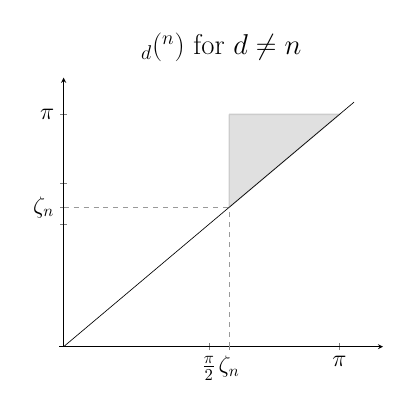
\begin{tikzpicture}[scale=0.6]
		\begin{axis} [
			title = {\LARGE $\barc\rH_d(\bS^n)$ for $d \neq n$},
			ticklabel style = {font=\Large},
			axis y line=middle,
			axis x line=middle,
			ytick={0.5,0.57,0.67,0.95},
			yticklabels={,$\zeta_n$,,$\pi$},
			xtick={0.5,0.57,0.95},
			xticklabels={$\frac{\pi}{2}$,$\zeta_n$, $\pi$},
			xmin=-0.015, xmax=1.1,
			ymin=0, ymax=1.1,]
			\addplot [thick,color=black!20!white,fill=black!30!white,
			fill opacity=0.4]coordinates {
				(0.57,0.95)
				(0.57,0.57)
				(0.95,0.95)
				(0.57,0.95)};
			\addplot [black!40!white,mark=none,dashed, thin] coordinates {(0,0.57) (0.57,0.57)};
			\addplot [black!40!white,mark=none,dashed, thin] coordinates {(0.57,0) (0.57,0.57)};
			\addplot [mark=none] coordinates {(0,0) (1,1)};
		\end{axis}
	\end{tikzpicture}
\end{tabular}
	% 	\caption{Estimation of the persistent homology barcode of $\bS^n$.
		% 	%Here, and throughout the paper, $\rH_\degp $ denotes $\degp$-homology.
		% 	We remark that for any \(n \in \N\) the value \(\zeta_n\) is bounded below by \(\pi/2\).}
	% 	\label{fig:Sk}
	% \end{figure}

%\subsubsection{}

For $n \in \N$ and $\ell_1, \dots, \ell_n \in \N^n$, let
\[
\VS^{\ell_1,\dots,\ell_n} =
\overbrace{\bS^1\vee\dots\vee\bS^1}^{\ell_1} \vee\dots\vee \overbrace{\bS^n\vee\dots\vee\bS^n}^{\ell_n}.
%(\bS^1)^{\vee m_1} \vee \dots \vee (\bS^n)^{\vee m_n}.
\]
Using the homotopy equivalence between the Vietoris--Rips filtration of a metric gluing with the wedge sum of the Vietoris--Rips filtration described in \cref{ss:wedge sum}, we have the following isomorphisms of persistence modules for \(\degp \in \N\) and \(\theta \in \cO(\ell,\degp)\):
\[
\begin{split}
	\rH_\degp (\VR\VS^{\ell_1,\dots,\ell_n}) &\cong \, \bigoplus_{i=1}^n \rH_\degp (\VR\bS^i)^{\oplus \ell_i}, \\
	\img_\theta \VR(\VS^{\ell_1,\dots,\ell_n}) &\cong \, \bigoplus_{i=1}^n (\img_\theta \VR\bS^i)^{\oplus \ell_i}.
\end{split}
\]

Therefore, both the homology barcodes and \(\img_\theta\)-barcodes of \(\VS^{\ell_1, \dots, \ell_n}\) are the multiset unions of the corresponding barcodes of \(\bS^1, \dots, \bS^n\); see \cref{fig:barcodes_vs}.
%To facilitate the bottleneck distance estimates in later sections, we illustrate the barcode estimates for the wedge sum of spheres in \cref{fig:barcodes_vs}.\anibal{More needs to be said in words. What does ``appropriate unions'' means? I also think the monotonicity of \(\zeta_n\) wrt \(n\) is important, no? \ling{It means taking unions degree-wise. I guess this is apparent, so I removed the word `appropriate'. The monotonicity does not really matter.}}

% $\rH_\degp(\VS^{\ell_1,\dots,\ell_n})$ contains $\ell_\degp$ copies of $(0,\zeta_\degp)$.
% All remaining bars in this barcode must be dominated by $(\zeta_n, \pi)$.
% This holds for all degrees, with the convention that $\ell_\degp = 0$ for $\degp > n$.

% Similarly, for any linear cohomology operation $\theta \in \cO(\ell,m)$ with $\ell \neq m$, every bar in either its $\img\theta$ or $\ker\theta$ barcode is dominated by $(\zeta_n, \pi)$.

\begin{figure}
	\centering
	\begin{tikzpicture}[scale=0.52]
	\begin{axis} [
		title = {\LARGE $\Hbarc[\field]{\degp}{\VS^n},1\leq \degp\leq n$},
		ticklabel style = {font=\Large},
		axis y line=middle,
		axis x line=middle,
		ytick={0.5,0.6,0.67,0.95},
		yticklabels={,$\zeta_\degp$,,$\pi$},
		xtick={0.5,0.55,0.95},
		xticklabels={$\frac{\pi}{2}$,$\zeta_n$, $\pi$},
		xmin=-0.015, xmax=1.1,
		ymin=0, ymax=1.1,]
		\addplot [mark=none] coordinates {(0,0) (1,1)};
		\addplot [thick,color=black!20!white,fill=black!30!white,
		fill opacity=0.4]coordinates {
			(0.55,0.95)
			(0.55,0.55)
			(0.95,0.95)
			(0.55,0.95)};
		\addplot [black!40!white,mark=none,dashed, thin] coordinates {(0,0.6) (0.6,0.6)};
		\addplot [black!40!white,mark=none,dashed, thin] coordinates {(0,0.55) (0.55,0.55)};
		\addplot [black!40!white,mark=none,dashed, thin] coordinates {(0.55,0) (0.55,0.55)};
		\addplot[barccolor,mark=*] (0, 0.6) circle (2pt) node[above right,barccolor]{};%{\Large\textsf{1}};
		%\node[mark=none] at (axis cs:0.68,0.21){$\Hbarc{2}{\VS^n}$};
	\end{axis}
\end{tikzpicture}
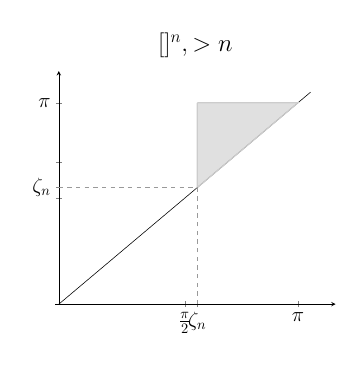
\begin{tikzpicture}[scale=0.52]
	\begin{axis} [
		title = {\LARGE $\Hbarc[\field]{\degp}{\VS^n}, \degp>n$},
		ticklabel style = {font=\Large},
		axis y line=middle,
		axis x line=middle,
		ytick={0.5,0.55,0.67,0.95},
		yticklabels={,$\zeta_n$,,$\pi$},
		xtick={0.5,0.55,0.95},
		xticklabels={$\frac{\pi}{2}$,$\zeta_n$, $\pi$},
		xmin=-0.015, xmax=1.1,
		ymin=0, ymax=1.1,]
		\addplot [mark=none] coordinates {(0,0) (1,1)};
		\addplot [thick,color=black!20!white,fill=black!30!white,
		fill opacity=0.4]coordinates {
			(0.55,0.95)
			(0.55,0.55)
			(0.95,0.95)
			(0.55,0.95)};
		\addplot [black!40!white,mark=none,dashed, thin] coordinates {(0,0.55) (0.55,0.55)};
		\addplot [black!40!white,mark=none,dashed, thin] coordinates {(0.55,0) (0.55,0.55)};
		%\node[mark=none] at (axis cs:0.68,0.21){$\Hbarc[\field]{\degp}{\VS^n}, \degp\geq 3$};
	\end{axis}
\end{tikzpicture}

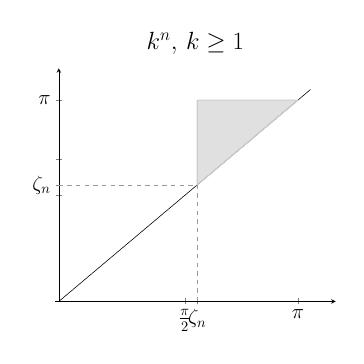
\begin{tikzpicture}[scale=0.52]
	\begin{axis} [
		title={\LARGE $\sqbarc{k}{\VS^n},\, k\geq 1$},
		ticklabel style = {font=\Large},
		axis y line=middle,
		axis x line=middle,
		ytick={0.5,0.55,0.67,0.95},
		yticklabels={,$\zeta_n$,,$\pi$},
		xtick={0.5,0.55,0.95},
		xticklabels={$\frac{\pi}{2}$,$\zeta_n$, $\pi$},
		xmin=-0.015, xmax=1.1,
		ymin=0, ymax=1.1,]
		\addplot [mark=none] coordinates {(0,0) (1,1)};
		\addplot [thick,color=black!20!white,fill=black!30!white,
		fill opacity=0.4]coordinates {
			(0.55,0.95)
			(0.55,0.55)
			(0.95,0.95)
			(0.55,0.95)};
		\addplot [black!40!white,mark=none,dashed, thin] coordinates {(0,0.55) (0.55,0.55)};
		\addplot [black!40!white,mark=none,dashed, thin] coordinates {(0.55,0) (0.55,0.55)};
		%\node[mark=none] at (axis cs:0.68,0.21){$\sqbarc{k}{\VS^n},\, k\geq 1$};
	\end{axis}
\end{tikzpicture}

	\caption{Let $\VS = \VS^{\ell_1,\dots,\ell_n}$ for some tuple of non-negative integers.
		\emph{Top row:} persistent homology barcodes of $\VS$, where the dot $(0,\zeta_m)$ has multiplicity $\ell_m$.
		\emph{Bottom row:} $\theta$-barcodes of $\VS$ where $\theta \in \cO(\ell,m)$ is any linear cohomology operation with \(\ell \neq m\).
        In each figure, the gray region represents where additional bars could exist within the corresponding barcode.}
	\label{fig:barcodes_vs}
\end{figure}